\documentclass[sigconf,nonacm]{acmart}
\settopmatter{printacmref=false}
\setcopyright{none}
\pagestyle{plain}

\AtBeginDocument{%
  \providecommand\BibTeX{{%
    \normalfont B\kern-0.5em{\scshape i\kern-0.25em b}\kern-0.8em\TeX}}}

\graphicspath{{images/}}

\begin{document}

\title{Sparse-Autoencoder Dissection of Emotion Features in Frozen Speech Encoders}

\author{Nima Kelidari}
\affiliation{\institution{USC ICT, Intelligent Human Perception Lab}\city{Los Angeles}\state{CA}\country{USA}}
\email{kelidari@usc.edu}
\author{Minoo Ahmadi}
\affiliation{\institution{USC ICT, Intelligent Human Perception Lab}\city{Los Angeles}\state{CA}\country{USA}}
\author{Chaitanya Parwatkar}
\affiliation{\institution{University of Southern California}\city{Los Angeles}\state{CA}\country{USA}}
\author{Xiangxu Lin}
\affiliation{\institution{University of Southern California}\city{Los Angeles}\state{CA}\country{USA}}
\renewcommand{\shortauthors}{Kelidari et al.}

\begin{abstract}
Linear probes show emotion is decodable in the middle-to-late layers of frozen speech transformers, but not which internal features carry it, nor whether the signal is acoustic or lexical. We train TopK Sparse Autoencoders (SAEs) on \emph{per-frame} activations of six frozen large encoders and dissect their emotion features on the lexicon-controlled CREMA-D corpus (91 actors $\times$ 12 fixed sentences $\times$ 6 emotions). A confound-controlled selection---a feature's firing must be more informative about emotion than about the spoken sentence or the speaker---isolates genuine emotion features from phonetic and speaker-driven ones. We find that (i) emotion \emph{disentangles} into clean monosemantic features earlier (L2--L7) than where it is best linearly \emph{decoded} (L10); (ii) all six encoders share an acoustic emotion-feature basis that generalizes across unseen speakers; and (iii) the recovered emotion signal is acoustic, not lexical. Decodability and disentanglement are thus distinct, and emotion in these encoders is carried by speaker-invariant acoustic features.
\end{abstract}

\keywords{speech emotion recognition, sparse autoencoders, mechanistic interpretability, probing, acoustic features}

\maketitle

\section{Introduction}
Self-supervised speech encoders dominate speech emotion recognition, yet were trained on ASR-style objectives that encode linguistic structure. Probing reveals \emph{where} emotion is readable, not \emph{which} features encode it or whether the signal is acoustic or lexical. Sparse autoencoders (SAEs) decompose dense activations into sparse, near-monosemantic features~\cite{gao2024scaling,saelens}, moving the analysis from decodability to mechanism. The fixed lexicon of CREMA-D~\cite{cao2014cremad} dissociates acoustic delivery from text by construction, so any recovered emotion signal there is necessarily acoustic.

\section{Method}
We re-extract \emph{un-pooled} per-frame hidden states from six frozen large encoders (HuBERT~\cite{hsu2021hubert}, WavLM, wav2vec2, w2v-BERT, MERT, Whisper~\cite{radford2023whisper}); the project's cached embeddings are mean-pooled, too few to train an over-complete SAE. CREMA-D layer~13 yields $940{,}273$ frames. We train a TopK SAE ($d_{\text{in}}{=}1024$, $d_{\text{sae}}{=}8192$, $k{=}32$, AuxK dead-feature revival), reaching FVU~$=0.070$ ($93\%$ variance explained), with $4/8192$ dead features.

Emotion features are scored by the mutual information (MI) between a feature's firing and the emotion label, thresholded at $5\sigma$ over a label-permutation null. \textbf{Confound control is decisive}: a feature qualifies only if $\mathrm{MI}(\text{emotion})$ exceeds both $\mathrm{MI}(\text{sentence})$ and $\mathrm{MI}(\text{actor})$, and it is monosemantic ($\geq 0.5$ activation mass on one emotion). Significance and monosemanticity alone flag $6407$ significant / $394$ monosemantic features, but $\sim$66\% carry more sentence (phonetic) or speaker information than emotion---the documented ``SAE rediscovers phonemes, not affect'' failure~\cite{saeasr2026}. After control, $61$ genuine emotion features remain (median monosemanticity $0.59$), dominated by anger and sadness; fear and neutral drop to zero. Acoustic-vs-lexical labeling uses cross-validated ROC-AUC of a logistic classifier predicting firing from eGeMAPS~\cite{eyben2016egemaps} (acoustic) vs.\ sentence identity (lexical); $R^2$ is unusable as the pooled features are $\sim$96\% sparse.

\begin{figure}[t]
  \centering
  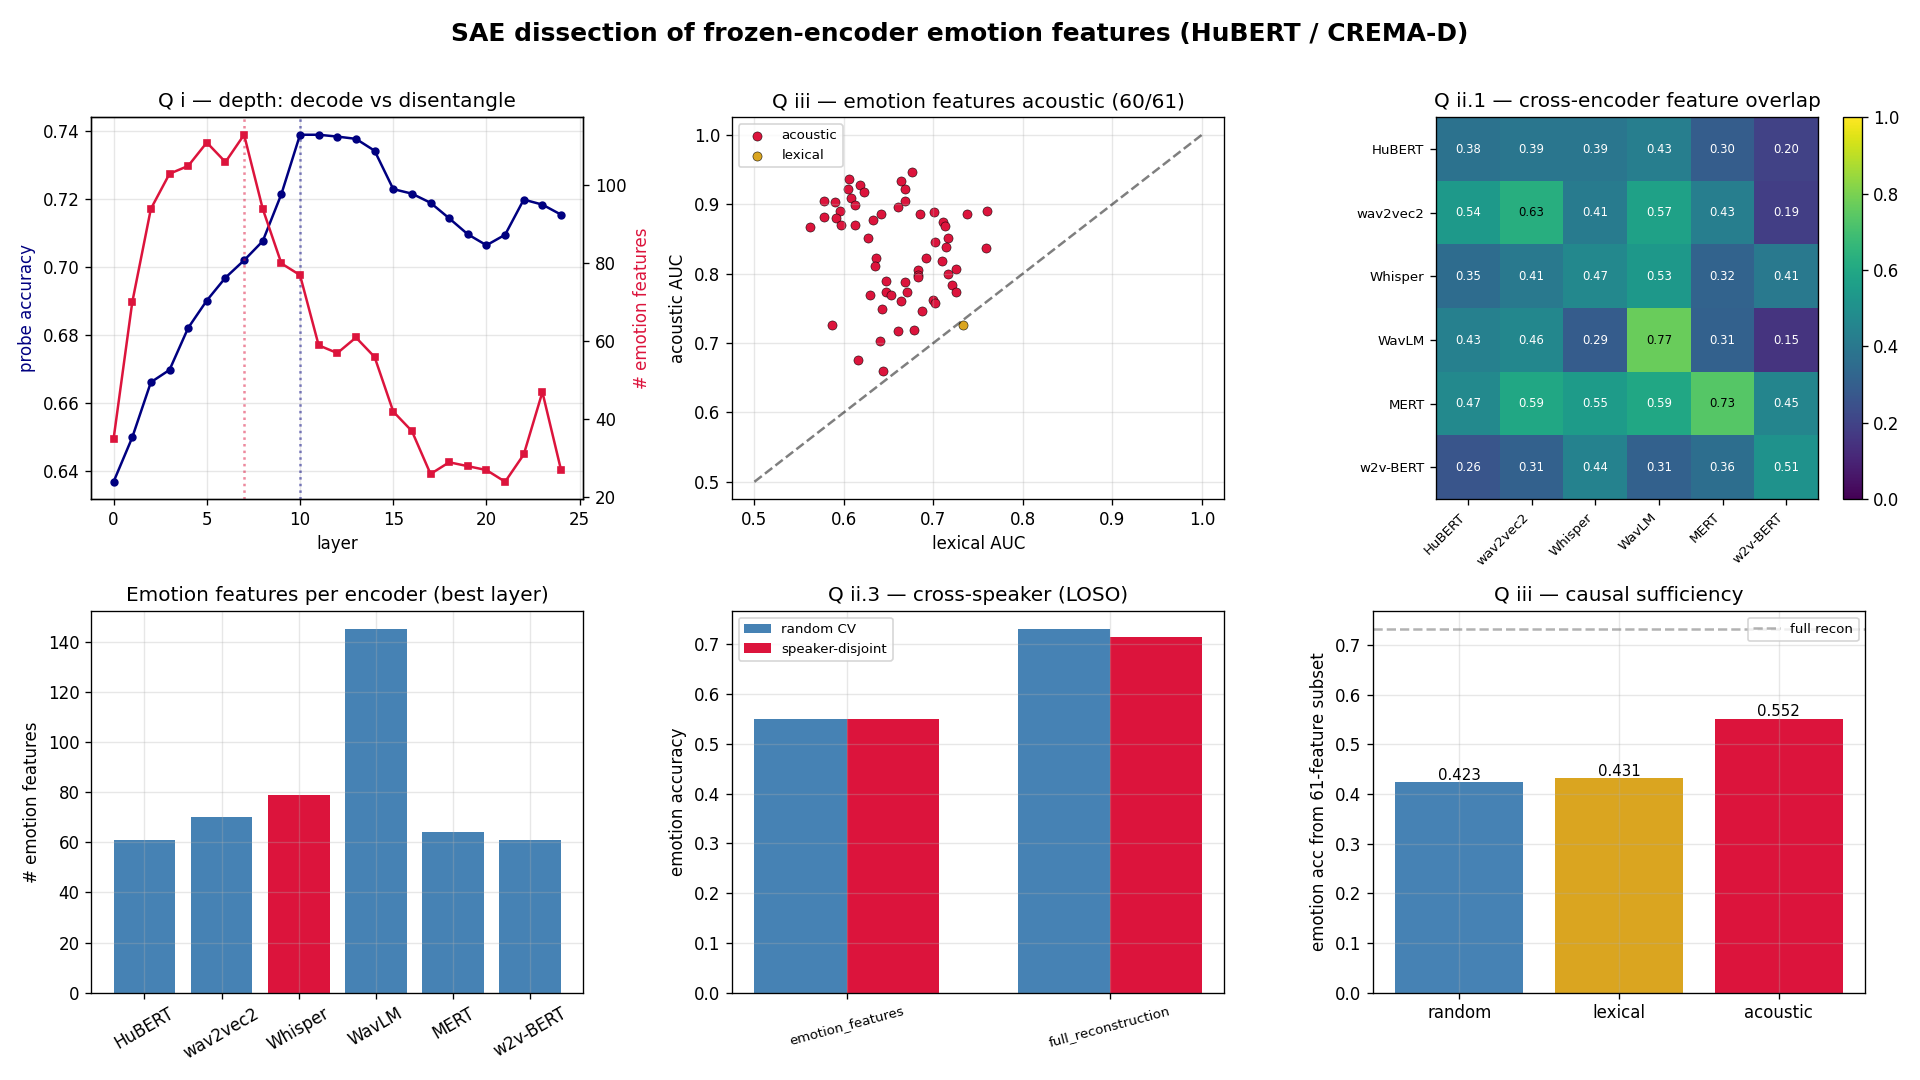
\includegraphics[width=\columnwidth]{fig_summary.png}
  \caption{SAE dissection (HuBERT/CREMA-D). Top: depth decode-vs-disentangle; acoustic vs lexical; cross-encoder overlap. Bottom: emotion features per encoder; cross-speaker (leave-speaker-out); causal sufficiency (acoustic vs lexical vs random).}
  \label{fig:summary}
\end{figure}

\section{Results}
\subsection{Depth: decode $\neq$ disentangle (Q\,i)}
A 25-layer sweep separates two curves (Fig.~\ref{fig:summary}, top-left). Linear probe accuracy peaks at L10 ($0.739$); the count of monosemantic emotion features peaks earlier at L7, and monosemanticity at L2. Deep layers (L17--24) retain decodability ($\sim$0.72) but lose disentanglement (24--47 features): emotion stays linearly readable while becoming distributed. \emph{Emotion organizes into clean features before the depth at which it is best decoded.}

\subsection{Generalization across paradigms and speakers (Q\,ii)}
All six encoders carry emotion features at their best layer (HuBERT~61, wav2vec2~70, Whisper~79, WavLM~145, MERT~64, w2v-BERT~61), all anger/sadness-dominated. Matching features across encoders by per-utterance firing correlation, Whisper$\rightarrow$SSL overlap ($0.40$) $\approx$ SSL$\rightarrow$SSL overlap ($0.39$): on fixed-lexicon CREMA-D Whisper is \emph{not} distinct, its known divergence concerning the lexical shortcut rather than acoustic emotion encoding. Under speaker-disjoint cross-validation over 91 actors, emotion accuracy is unchanged (random $0.551$ vs.\ disjoint $0.551$; leave-speaker-out drop $\approx 0$) and each feature fires for $\sim$95\% of its emotion's actors. Because selection excluded speaker-entangled features, the published MESD leave-one-speaker-out collapse ($\sim$0.30) is attributable to exactly those excluded features.

\subsection{Acoustic, not lexical (Q\,iii)}
The positive control (fixed lexicon $\Rightarrow$ must be acoustic) labels $60/61$ emotion features acoustic (eGeMAPS firing-AUC $0.83$ vs.\ sentence AUC $0.66$). Causally (Fig.~\ref{fig:summary}, bottom-right), emotion decodes from the $61$ acoustic features at $0.552$, vs.\ $0.431$ from lexical and $0.423$ from random features (6-class; full reconstruction $0.73$). The recovered emotion signal is acoustic.

\begin{table}[t]
  \caption{Key numbers (HuBERT / CREMA-D).}
  \label{tab:key}
  \small
  \begin{tabular}{ll}
    \toprule
    Quantity & Value \\
    \midrule
    SAE FVU (variance explained) & $0.070$ ($93\%$) \\
    Dead features & $4/8192$ \\
    Emotion features (sig $\to$ mono $\to$ confound) & $6407 \to 394 \to 61$ \\
    Decode peak / disentangle peak layer & L10 / L7 \\
    Acoustic features (positive control) & $60/61$ \\
    Sufficiency acoustic / lexical / random & $0.552 / 0.431 / 0.423$ \\
    Cross-speaker leave-speaker-out drop & $\approx 0$ \\
    \bottomrule
  \end{tabular}
\end{table}

\section{Discussion and Limitations}
Decodability and disentanglement are distinct axes: a probe reads emotion best where the representation is linearly separable, but the encoder packs emotion into clean monosemantic features earlier. On lexicon-controlled data all encoders converge on a shared acoustic basis whose features survive speaker-disjoint evaluation; the Whisper-vs-SSL divergence is about exploiting a lexical shortcut when one exists~\cite{ma2026lora}, which CREMA-D cannot pose and which the deferred EMIS experiment targets. Utterance-pooled sparse features make necessity-ablation of small subsets near-null (the signal is distributed), so sufficiency is the informative test. The IEMOCAP real-transcript ablation, the SpeechCraft cross-lingual arm, and the EMIS audio-vs-text separation are deferred (data unavailable on our cluster) with runnable stubs.

\bibliographystyle{ACM-Reference-Format}
\bibliography{references}

\end{document}
